% 第 5 章 Using Flyline Analysis Tools
\bichapter{使用飞线分析工具}{Using Flyline Analysis Tools}
\label{chap:gui-fly}

IC Compiler II GUI 提供一组工具，在版图（layout）中用飞线（flyline）查看线网连接（net connection）、穿越路径（feedthrough path）、时序路径（timing path）以及其他路径信息。

下列主题说明 GUI 所支持的设计规划任务：
\begin{itemize}
  \item 线网连接飞线
  \item 路径分析器飞线
  \item 数据流飞线
  \item 寄存器追踪飞线
  \item 时钟主干规划飞线
\end{itemize}

\section{线网连接飞线}
\subsection*{Net Connections Flylines}

IC Compiler II 工具提供 Net Connections Flylines 工具，用于查看设计中层次（hierarchy）、宏单元（macro）、标准单元（standard cell）与端口（port）之间的线网连接。可用该工具查看这些对象之间的连接数量，并追踪单条线网。要打开 Net Connections Flylines 面板，选择 \textbf{View > Flylines > Net Connections}，或单击 Net Connections Flylines 按钮。Net Connections Flylines 面板见图~\ref{fig:gui-77}。

\begin{figure}[htbp]
\centering
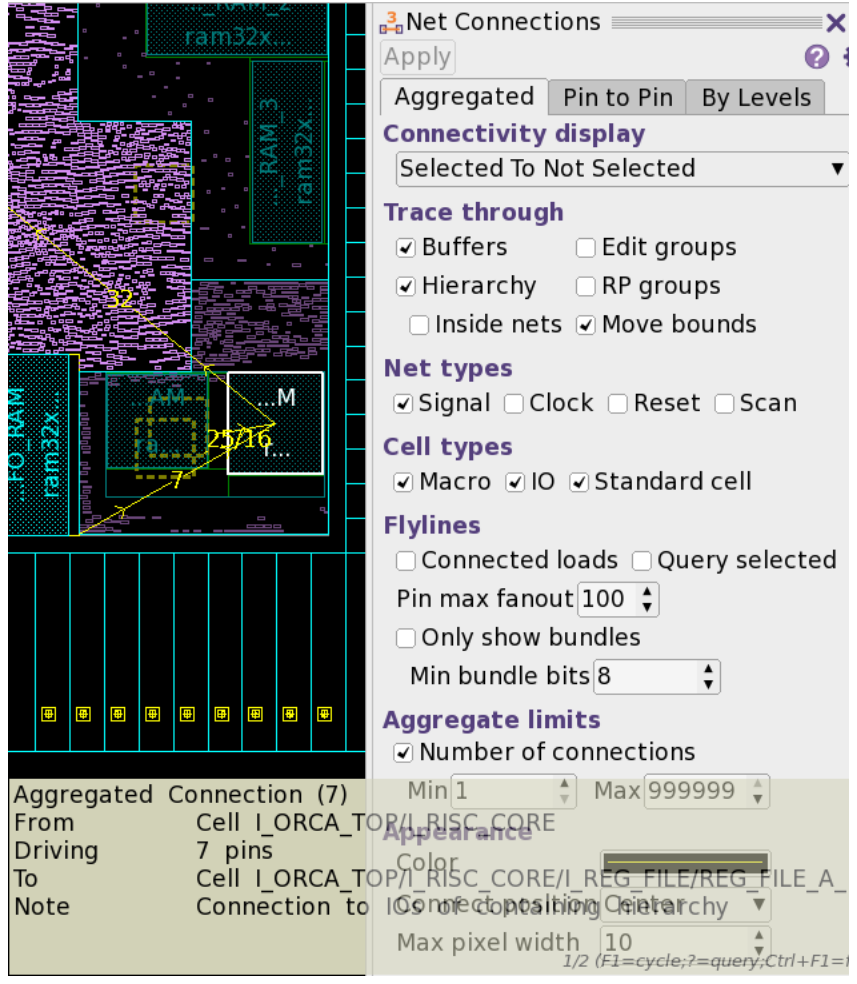
\includegraphics[width=0.92\textwidth]{gui-fig-077.png}
\caption{线网连接飞线面板}
\label{fig:gui-77}
\end{figure}

\subsection{飞线显示模式}
\subsubsection*{Flyline Display Modes}

Net Connections 面板支持下列飞线显示模式：
\begin{itemize}
  \item Aggregated（默认）
  \item Pin to Pin
  \item By Levels
\end{itemize}

这些模式分述如下。使用某一模式时，先单击面板顶部相应的选项卡（Aggregated、Pin to Pin 或 By Levels），再单击 Apply。

\subsection{管脚到管脚飞线}
\subsubsection*{Pin to Pin Flylines}

在 Pin to Pin 模式下，工具为各个管脚（pin）显示飞线。若起始管脚是驱动管脚（driver pin），飞线从每个起始管脚画到全部已追踪的负载管脚（load pin）。若起始管脚是负载管脚，工具则把飞线画到全部已追踪的驱动管脚。

\subsection{按级数}
\subsubsection*{By Levels}

在 By Levels 模式下，工具按 Driver 与 Load 选项所指定的追踪深度显示飞线。除缓冲器单元（buffer）外，工具把每个标准单元计为一级。若选中 \opt{Ignore buffers}，缓冲器不计入级数。此模式还支持为所选驱动管脚与负载管脚使用不同的飞线颜色。

单击一条聚合飞线（aggregated flyline），可以下钻并查看单条飞线的细节。工具打开 Net Connections Explorer 对话框，并显示该聚合飞线所代表的线网列表。Net Connections Explorer 对话框的进一步说明见第~\ref{sec:gui-fly-explorer}~节。要查看单条飞线，也可以取消选中 \opt{Aggregate by block}。取消该选项后，工具用单条飞线替换聚合飞线。

\begin{noteBox}
工具根据路径上所选的管脚以及所选对象的类型来显示飞线。所选管脚是否位于层次边界上，显示的飞线也会不同。
\end{noteBox}

\subsection{聚合飞线}
\subsubsection*{Aggregated Flylines}

在 Aggregated 飞线模式下，工具按飞线驱动管脚与负载管脚的父层次单元、移动约束（move bound）、编辑组（edit group）、相对布局组（RP group）或电压区（voltage area）对这些管脚分组。聚合飞线显示为一条线，并带有负载管脚和（或）驱动管脚的计数。该计数显示在每一对唯一相连父对象的中心。要显示哪些父对象类型，由所选的 Trace through 选项决定。若某类穿越追踪对象未在面板中选中，则仍把它作为一种可能的父对象类型。若最初选中的对象是编辑组、RP 组、移动约束或电压区，则这些对象类型也属于候选父对象类型。

\subsection{设置飞线显示选项}
\subsubsection*{Setting Flyline Display Options}

用 Connectivity Display 选项，按所选对象更改所显示的连接：
\begin{itemize}
  \item \opt{Selected to All}：显示任意选中对象与任何其他对象之间的飞线。
  \item \opt{Selected to Selected}：只显示选中对象之间的飞线。
  \item \opt{Selected to Not Selected}：若只选中一个对象，显示该选中对象与任何其他对象之间的飞线；若选中两个或更多对象，显示从每个并未连接到另一选中对象的选中对象出发的飞线。
\end{itemize}

用 Trace through 选项控制线网如何追踪：
\begin{itemize}
  \item \opt{Buffers}：选中此选项后，继续穿过缓冲器单元追踪，直到到达非缓冲器单元。取消选中后，工具在到达缓冲器单元或任何其他单元时停止追踪。
  \item \opt{Hierarchy}：选中此选项后，继续穿过层次管脚追踪。取消选中后，工具在到达层次管脚时停止追踪。
  \item \opt{Edit groups}：选中此选项后，在编辑组边界处停止追踪。取消选中后，追踪时忽略编辑组。
  \item \opt{RP groups}：选中此选项后，在 RP 组边界处停止追踪。取消选中后，追踪时忽略 RP 组。
  \item \opt{Inside nets}：选中此选项后，追踪块内部的线网。默认追踪块外部的线网。此选项可与 Pin to Pin 选项卡中的 \opt{Through points} 选项组合使用，以便在选中某个块管脚时追踪穿越连接（feedthrough connection）。
  \item \opt{Move bounds}：禁用此选项时，追踪在连接移动约束边界上管脚的线网处停止。当移动约束内部的单元连接到移动约束外部的单元时，即形成该边界。若选中移动约束内部的单元，工具不把飞线追踪到移动约束外部的单元。若选中移动约束外部的单元，工具不把飞线追踪到移动约束内部的单元。默认选中此选项，工具会穿过移动约束继续追踪。
\end{itemize}

用 Net Types 选项指定要追踪的线网类型：\opt{Signal}、\opt{Clock}、\opt{Reset}、\opt{Scan}、\opt{Tie High} 与 \opt{Tie Low}。

用 Cell Types 选项指定要追踪的一种或多种单元类型：宏单元、I/O 或标准单元。

用 Flylines 选项进一步控制显示哪些飞线：
\begin{itemize}
  \item \opt{Connected loads}：选中此选项后，显示两个负载之间的飞线。取消选中后，工具只显示驱动与负载之间的飞线。
  \item \opt{Query selected}：选中此选项后，单击对象时更新 Query 面板。该面板显示当前所显示飞线的源、目标以及连接数量。
  \item \opt{Pin max fanout}：隐藏扇出（fanout）大于指定数值的飞线。
  \item \opt{Only show bundles}：选中此选项后，只显示束信号（bundle）的飞线。
  \item \opt{Min bundle pins}：隐藏管脚数少于指定数值的束的飞线。
\end{itemize}

用 Aggregated Connections 选项按连接数控制聚合飞线的显示：
\begin{itemize}
  \item \opt{Number of connections}：选中此选项后，用 Min 与 Max 设置过滤聚合飞线；若总连接数超出指定范围，则隐藏该聚合飞线。
  \item \opt{Min}：在已选中 \opt{Number of connections} 且总连接数小于指定值时，隐藏该聚合飞线。
  \item \opt{Max}：在已选中 \opt{Number of connections} 且总连接数大于指定值时，隐藏该聚合飞线。
\end{itemize}

用 Include 选项控制所追踪的单元类型：
\begin{itemize}
  \item \opt{Macros}：选中此选项后，追踪中包含宏单元。
  \item \opt{IOs}：选中此选项后，追踪中包含 I/O 单元。
  \item \opt{Standard cells}：选中此选项后，追踪中包含标准单元。
\end{itemize}

用 Appearance 选项控制飞线的宽度与位置：
\begin{itemize}
  \item \opt{Connect Position}：指定飞线起点或终点的绘制位置，可选 center、inside、lower left、lower right、upper left 或 upper right。
  \item \opt{Max pixel width}：把飞线的绘制宽度限制为指定的像素数。
  \item \opt{Nets per pixel}：按线网连接数指定飞线宽度。例如设置为 100 nets/pixel，而某条线网连接含有 300 条连接时，工具绘制 3 像素宽的线（300 条线网 / 每像素 100 条线网 = 3 像素）。
  \item \opt{Color}：指定飞线的颜色。
\end{itemize}

\subsection{显示到布线通道的连接}
\subsubsection*{Displaying Connections to Route Corridors}

选中一条布线通道（route corridor）时，工具取得该布线通道所对应线网的管脚，并从管脚中心向布线通道形状的最近边绘制飞线。若布线通道中含有连接到该布线的中间单元，工具用另一种颜色向这些单元绘制飞线。

\subsection{线网连接浏览器}
\label{sec:gui-fly-explorer}
\subsubsection*{Net Connections Explorer}

使用 Net Connections Explorer 查询聚合飞线中的单条线网，或在单条飞线中显示各条线段网。单击任意飞线即可打开该对话框。对话框显示源块或源单元、目标块或目标单元，以及该飞线所代表的线网列表。可以单击 From: 或 To: 文本后面的名称，以选中对应的块、单元或端口。将指针移到对话框右上角的 Info 图标上，可查看对话框中所显示线网连接的摘要信息。

\begin{figure}[htbp]
\centering
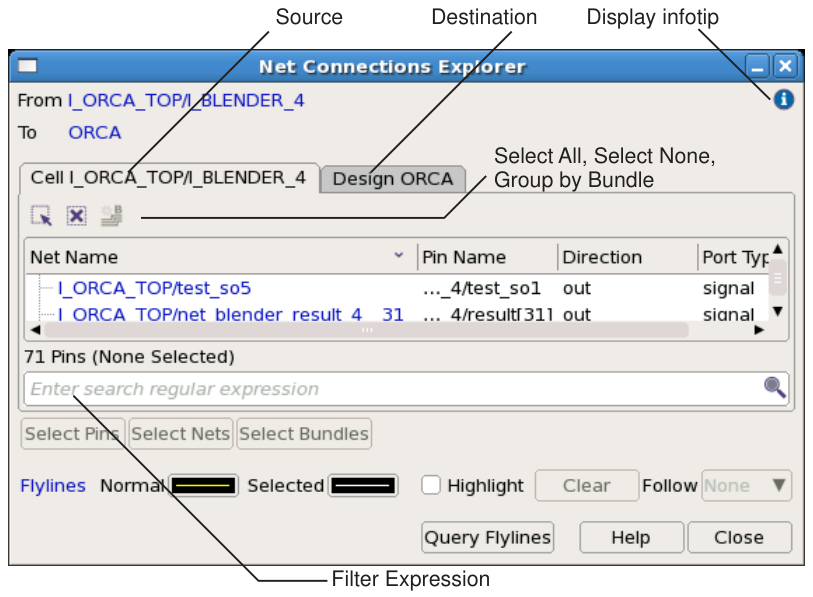
\includegraphics[width=0.92\textwidth]{gui-fig-078.png}
\caption{线网连接浏览器的聚合飞线模式}
\label{fig:gui-78}
\end{figure}

对话框显示两个选项卡：一个选项卡包含源对象的管脚与线网，另一个选项卡包含目标对象的管脚与线网。单击相应选项卡，即可显示与该对象关联的线网和管脚。

要过滤线网列表，在框中输入过滤表达式。表达式可以是简单匹配表达式，也可以是 Tcl 正则表达式。默认把过滤表达式应用于线网名。要对管脚名应用该表达式，使用语法 \cmd{"Pin Name:string"}，其中 \cmd{string} 是搜索表达式，\cmd{Pin Name} 是该列的列标题。

单击 Select Pins 或 Select Nets 按钮，在版图中选中高亮线网的管脚或线网。单击 Select Bundles，选中高亮线网对应的线网束。

要更改未选中飞线或已选中飞线的颜色，单击 Normal 右侧或 Selected 右侧的飞线颜色框。要让先前选中的飞线继续显示在版图中，选中 Highlight。要清除先前显示的飞线，单击 Clear。

用 Follow 设置控制工具如何把所选飞线放到视图中心。要保持同一缩放比例，并把版图平移到使所选飞线位于视图中心，在 Follow 框中选择 Pan。要平移版图并放大，使飞线适合视图，在 Follow 框中选择 Zoom。

追踪单条飞线时，显示如图~\ref{fig:gui-79} 所示。

\begin{figure}[htbp]
\centering
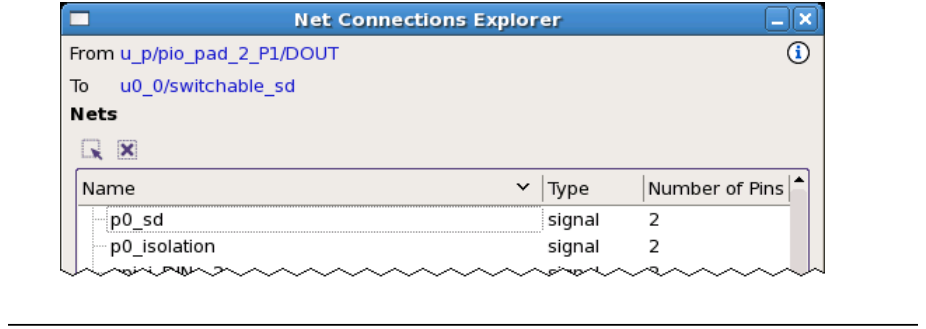
\includegraphics[width=0.92\textwidth]{gui-fig-079.png}
\caption{线网连接浏览器的单条飞线模式}
\label{fig:gui-79}
\end{figure}

要在 Query 面板中显示当前飞线连接列表，单击 Query Flylines。要查看 Net Connections Explorer 对话框的帮助信息，单击 Help。

\section{路径分析器飞线}
\subsection*{Path Analyzer Flylines}

IC Compiler II 工具支持 Path Analyzer Flylines 工具，用于查看设计中顶层信号（top-level signal）、宏单元、端口与层次之间的时序路径连接。使用 Path Analyzer Flylines 工具，可以识别可能与版图有关的时序问题，并交互分析布局对时序的影响。该工具提供两种分析模式，即连接模式（connection mode）与时序模式（timing mode），用来决定飞线优先显示哪些信息。要打开 Path Analyzer Flylines 面板，选择 \textbf{View > Flylines > Path Analyzer Flylines}，或单击 Path Analyzer Flylines 按钮。Path Analyzer Flylines 面板见图~\ref{fig:gui-80}。

\begin{figure}[htbp]
\centering
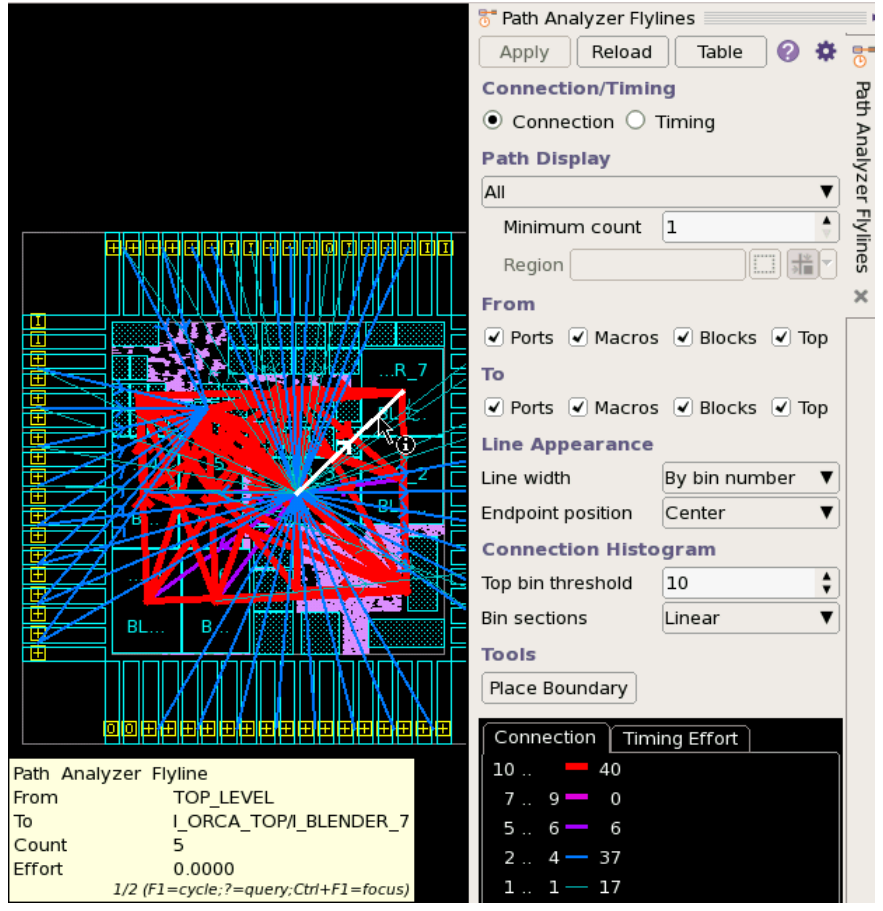
\includegraphics[width=0.92\textwidth]{gui-fig-080.png}
\caption{路径分析器飞线面板}
\label{fig:gui-80}
\end{figure}

单击面板顶部的 Reload 按钮，重新加载飞线。

若版图中含有模块边界（module boundary），单击 Tools 区中的 Place Boundary 按钮，把当前显示的模块边界放到块版图显示上。工具把每个模块边界居中放在该模块标准单元的位置上。工具用画到模块边界的飞线表示与标准单元的连接，模块内部所含的宏单元与层次块不参与这一表示。与宏单元的连接用直接连到宏单元的飞线表示，而不连到模块边界。若某个模块不含标准单元，模块边界放在坐标 (0,0)，并且不向该模块边界绘制飞线。

模块边界提供设计层次中单元物理位置的信息。可以用 Hierarchy Browser 创建模块边界，并与 Path Analyzer Flylines 工具一起使用。当飞线连接到模块边界内的某个单元时，Path Analyzer Flylines 工具把飞线画到模块边界。若不存在模块边界，Path Analyzer Flylines 工具把飞线画到块的中心。要检查层次，选择 \textbf{View > Hierarchy Browser} 启动 Hierarchy Browser 工具。

\subsection{按连接数查看时序路径}
\label{sec:gui-fly-bycount}
\subsubsection*{Viewing Timing Paths by Number of Connections}

单击 Reload 按钮后，Connection/Timing 区中的 Connection 模式默认处于选中状态。Connection 模式显示设计中端口、模块与宏单元之间的时序路径连接飞线。工具按连接数对飞线分档（binning）并分组；连接数最多的飞线显示为红色。若只看到浅蓝色飞线，可在 Line Appearance 区更改 \opt{Threshold for Top Bin} 的值来调整分档。

若看到跨越很长距离的红色或亮紫色飞线，可能需要修改布图规划（floorplan）以缩短这些路径。大量长路径会造成布线拥塞（routing congestion），并在对块做时序分析时加重总负裕量（total negative slack，TNS）问题。

将鼠标指针移到飞线上，可查看更多信息。工具显示信息提示（infotip），如图~\ref{fig:gui-81}；此例中，高亮飞线的全部路径方向相同。信息提示显示路径终点（endpoint）、两个对象之间的飞线计数，以及优化这些路径时序所需的相对时序努力。若该努力大于 1.0，对该路径做时序收敛时可能会遇到困难。

\begin{figure}[htbp]
\centering
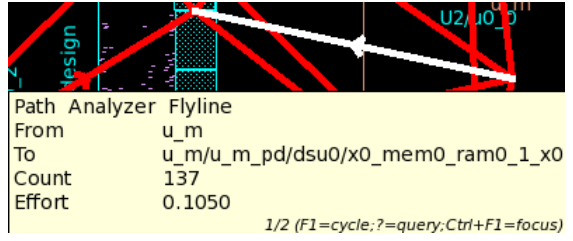
\includegraphics[width=0.92\textwidth]{gui-fig-081.png}
\caption{带信息提示的单向飞线}
\label{fig:gui-81}
\end{figure}

图~\ref{fig:gui-82} 是信号沿两个方向传输的飞线。飞线上不显示方向箭头。信息提示把信号计数显示为 \cmd{Total - (endpoint1 to 2 + endpoint2 to 1)}，把 Effort 显示为 \cmd{Total maximum - max of (endpoint1 to 2 max to endpoint2 to 1 max)}。

\begin{figure}[htbp]
\centering
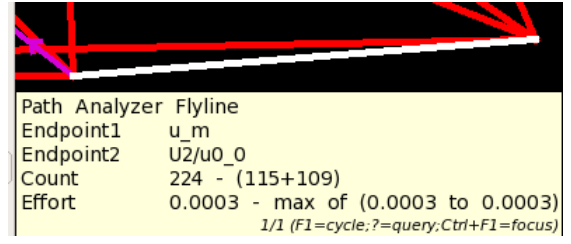
\includegraphics[width=0.92\textwidth]{gui-fig-082.png}
\caption{混合方向的飞线}
\label{fig:gui-82}
\end{figure}

单击飞线可展开该飞线，并查看对象之间的各条连接。工具为每条时序路径显示一条飞线，如图~\ref{fig:gui-83}。要去掉这些细节飞线，另选一个对象，或单击版图外部。

\begin{figure}[htbp]
\centering
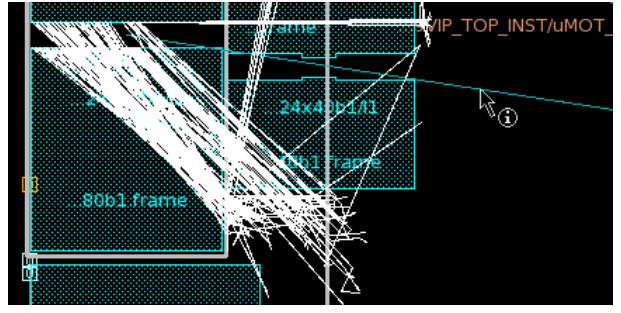
\includegraphics[width=0.92\textwidth]{gui-fig-083.png}
\caption{详细连接飞线}
\label{fig:gui-83}
\end{figure}

若只查看经过设计中某一区域的飞线，在 Path Display 框中选择 Region，并单击图~\ref{fig:gui-84} 所示的虚线方块按钮。用鼠标在版图上绘制矩形，指定分析区域。工具去掉不经过该区域的飞线。

\begin{figure}[htbp]
\centering
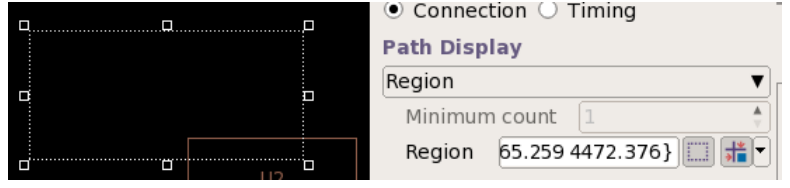
\includegraphics[width=0.92\textwidth]{gui-fig-084.png}
\caption{创建区域矩形}
\label{fig:gui-84}
\end{figure}

过滤飞线的进一步说明见第~\ref{sec:gui-fly-filter}~节。

\subsection{按关键程度查看时序路径}
\subsubsection*{Viewing Timing Paths by Criticality}

在 Connection/Timing 区选择 Timing，显示设计中各对象之间时序最关键路径的时序路径连接飞线。在时序模式下，工具按连接的关键程度（criticality）对飞线分档，并把最关键的飞线显示为红色。按第~\ref{sec:gui-fly-bycount}~节所述，将指针移到飞线上并单击飞线，可查看这些飞线的更多信息。

用 Distance Sensitivity 框控制计算优化努力时对飞线长度所加的权重。更改 Distance Sensitivity 后，工具重新计算该飞线的优化努力。Distance Sensitivity 的值越大，工具对较长飞线所加的权重越大。更新后的努力值可在信息提示中查看。

一般而言，线电阻（wire resistance）较高的工艺可能需要较高的 Distance Sensitivity 设置。若只有在灵敏度很高（7 或更大）时才出现红色飞线，则该设计很可能没有时序问题。

\subsection{更改飞线显示}
\subsubsection*{Changing the Flyline Display}

单击 Display 选项卡，查看并修改 Path Analyzer Flylines 显示的线宽与分档设置。选中 \opt{Apply line widths}，按对象之间的连接数更改飞线线宽。选中 \opt{Log Scale}，把分档改为使用对数刻度（logarithmic scale），而不使用线性刻度（linear scale）。在 \opt{Threshold for Top Bin} 框中输入新值，设置最高档的最大值。

在连接模式下，Display 选项卡用颜色表示每条飞线的相对连接数。若选中 \opt{Apply line widths}，工具用不同线宽显示飞线，最高档使用最宽的线。

在时序模式下，颜色表示时序飞线的关键程度。若选中 \opt{Apply line widths}，工具用不同线宽表示相对连接数，最宽的线表示连接数最多。

\subsection{按设计对象及其他约束过滤}
\label{sec:gui-fly-filter}
\subsubsection*{Filtering by Design Object and Other Constraints}

在 From 与 To 设置区中选中要分析的对象类型。在 Path Display 框中选择一项，指定创建飞线时使用的源对象与目标对象：
\begin{itemize}
  \item \opt{All}：显示飞线，不附加任何选择条件。From 与 To 设置处于启用状态。
  \item \opt{Region}：显示经过用户指定矩形的飞线。From 与 To 设置处于启用状态。
  \item \opt{Selected From/To All}：显示以选中对象为起点或终点、并连到任何其他对象的飞线。From 与 To 设置处于禁用状态。
  \item \opt{Selected to Selected}：显示以选中对象为起点或终点的飞线。From 与 To 设置处于禁用状态。
  \item \opt{All to Selected}：显示从任意对象开始、并在选中对象处结束的飞线。From 与 To 设置处于禁用状态。
  \item \opt{Selected to All}：显示从选中对象开始、并在任何其他对象处结束的飞线。From 与 To 设置处于禁用状态。
\end{itemize}

\subsection{在表中查看时序路径信息}
\subsubsection*{Checking Timing Paths Info in Table}

单击控制板（palette）顶部的 Table 按钮，在表中显示飞线终点、连接计数与时序努力。图~\ref{fig:gui-85} 是一个示例表。

\begin{figure}[htbp]
\centering
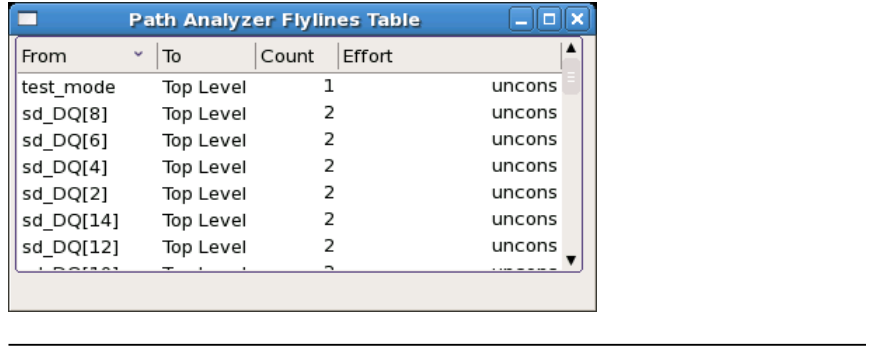
\includegraphics[width=0.92\textwidth]{gui-fig-085.png}
\caption{路径分析器飞线表}
\label{fig:gui-85}
\end{figure}

\subsection{路径分析器飞线最佳实践}
\subsubsection*{Path Analyzer Flylines Best Practices}

使用 Path Analyzer Flylines 工具时，可参考下列建议：
\begin{itemize}
  \item 对大多数应用，应取消选中 From 与 To 区中的 \opt{Top}，以去掉不连接到任何特定宏单元或模块边界的飞线。这样更容易看清其余飞线和其他信息。
  \item 在连接模式下，输入大于零的 \opt{Minimum count} 值，指定对象之间至少要有多少条连接才显示飞线。
  \item 在时序模式下，切换 Path Display 区中的 \opt{Unconstrained}，以包含没有时序约束的时序路径飞线，也就是努力为 0 的路径。切换 \opt{Unachievable}，以包含无法满足当前时序约束的路径飞线，也就是努力为 10 或更大的路径。在 \opt{Minimum Effort} 中输入最低努力级别，以隐藏努力级别小于或等于该指定值的路径。
\end{itemize}

\section{数据流飞线}
\subsection*{Data Flow Flylines}

使用 Data Flow Flylines 工具查看宏单元、块、模块边界与 I/O 端口之间的连接。该工具帮助理解宏单元布局质量，并查看设计中的宏单元到宏单元路径。要打开 Data Flow Flylines 面板，选择 \textbf{View > Flylines > Data Flow Flylines}，或单击 Data Flow Flylines 按钮。

\begin{figure}[htbp]
\centering
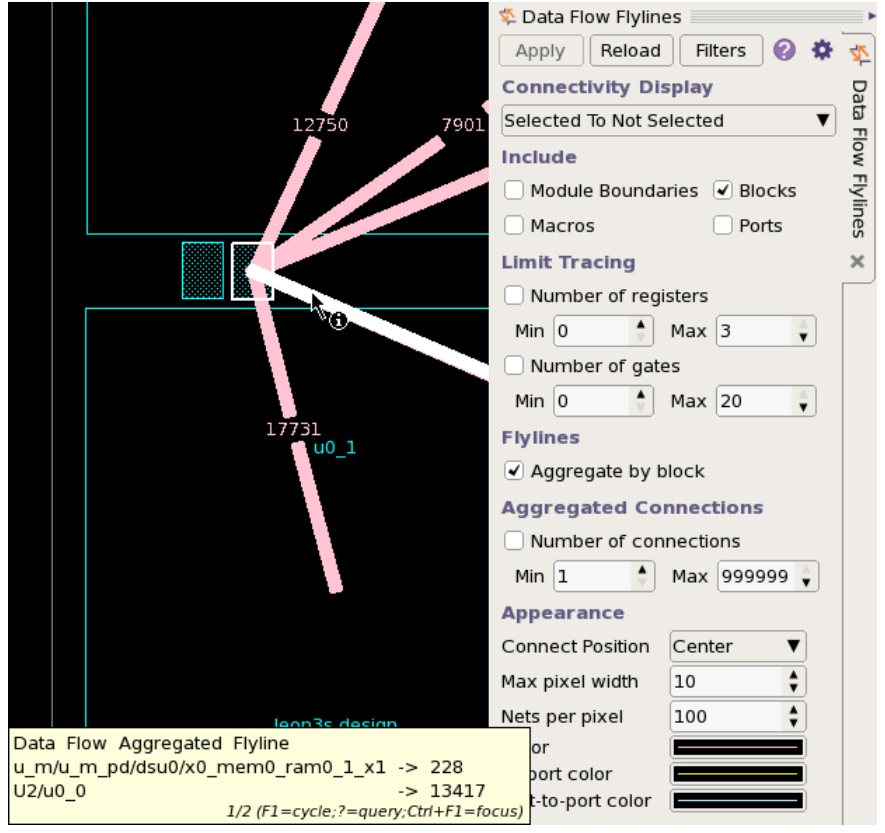
\includegraphics[width=0.92\textwidth]{gui-fig-086.png}
\caption{数据流飞线面板}
\label{fig:gui-86}
\end{figure}

本节包括以下内容：
\begin{itemize}
  \item 计算数据流飞线
  \item 追踪飞线
  \item 设置追踪选项
  \item 查看飞线细节并过滤飞线
  \item 数据流飞线的管脚与线网过滤器
  \item 用 Tcl 命令分析数据流飞线
  \item 保存与恢复数据流飞线连接数据
\end{itemize}

\subsection{计算数据流飞线}
\label{sec:gui-fly-compute}
\subsubsection*{Computing Data Flow Flylines}

追踪飞线之前，必须先计算飞线，以便把它们载入工具，步骤如下：
\begin{enumerate}
  \item 单击 Data Flow Flylines 面板上的 Reload 按钮。
  \item 在 Compute Data Flow Flylines 对话框中，选择要追踪的寄存器（register）级数、门（gate）级数和最大扇出。
  \item 单击 Filters 按钮，指定追踪期间要忽略的线网和管脚。进一步说明见第~\ref{sec:gui-fly-pinnet}~节。
  \item 单击 OK，计算数据流飞线。
\end{enumerate}

\subsection{追踪飞线}
\subsubsection*{Tracing Flylines}

初始化数据流飞线之后，可以在版图窗口中交互追踪飞线。典型流程包括以下步骤：
\begin{enumerate}
  \item 单击某个宏单元、块、模块边界或 I/O 端口以选中它；工具显示到 Include 区中所选对象的飞线连接。
  \item 将指针移到飞线上，在信息提示中查看连接数。
  \item 单击该飞线，打开 Data Flow Connections and Filters 对话框。对话框显示该飞线所代表的连接列表，进一步说明见第~\ref{sec:gui-fly-details}~节。
  \item 单击列表中的一条路径，显示该路径的飞线。
  \item 单击 ([+]) 按钮展开该路径，再单击代表路径中某一段的一行；工具用红色显示该段的详细路径飞线。
  \item 继续单击路径中的其他段进行追踪，或按上箭头键或下箭头键，在段列表中滚动。
\end{enumerate}

\subsection{设置追踪选项}
\subsubsection*{Setting Tracing Options}

Data Flow Flylines 工具提供控制飞线追踪的选项。用 Connectivity Display 设置控制显示哪些连接：
\begin{itemize}
  \item \opt{All}：显示全部路径。
  \item \opt{Selected To All}：显示从选中对象到全部相连对象的路径。
  \item \opt{Selected To Selected}：显示从选中对象到其他已连接的选中对象的路径。
  \item \opt{Selected To Not Selected}：显示从选中对象到已连接但未被选中的对象的路径。
\end{itemize}

用 Include 区选择追踪时要包含的对象类型。

用 Limit Tracing 区调整飞线中包含的寄存器数量和门数量。只能在 Compute Data Flow Flylines 对话框里已指定的级数之内减少级数；要增加可用级数，单击 Reload 并重新计算飞线。

\begin{noteBox}
默认情况下，源管脚与目标管脚之间最小门数和最大门数的计数不包含缓冲器与反相器（inverter）。因此，详细路径连接所显示的门数可能多于预期。
\end{noteBox}

聚合连接是把源对象与目标对象相同的飞线合并为一条飞线。要更改聚合飞线的行为：
\begin{itemize}
  \item 选中或取消选中 \opt{Aggregate}，以显示聚合飞线或显示单条飞线。
  \item 选中 \opt{Number of connections}，并为聚合飞线选择最小连接数与最大连接数；连接数超出该范围的聚合飞线会被工具隐藏。
\end{itemize}

用 Appearance 区更改飞线的连接点、线宽和颜色：
\begin{itemize}
  \item 在列表中选择一项 \opt{Connect Position}，更改飞线在版图中的绘制位置；工具把飞线画到对象上的指定位置。
  \item 用 \opt{Max pixel width} 设置把飞线的绘制宽度限制为指定的像素数。
  \item 用 \opt{Nets per pixel} 设置按线网连接数指定飞线宽度。例如设置为 100 nets/pixel，而某条线网连接含有 300 条连接时，得到 3 像素宽的线（300 / 100 = 3）。
  \item 用 \opt{Color} 设置更改宏单元、块与模块边界之间飞线的显示颜色。
  \item 用 \opt{To port color} 设置更改连到端口的飞线颜色。
  \item 用 \opt{Port-to-port color} 设置更改端口到端口飞线的颜色。
  \item Wire length 是所选对象的飞线总长度，由工具自动计算。
\end{itemize}

\subsection{查看飞线细节并过滤飞线}
\label{sec:gui-fly-details}
\subsubsection*{Viewing Flyline Details and Filtering Flylines}

使用 Data Flow Connections and Filters 对话框，查看聚合飞线内部的各条连接、查看单条飞线，或设置追踪飞线时使用的管脚过滤器与线网过滤器。要打开此对话框，单击 Data Flow Flylines 工具生成的聚合飞线。

\begin{noteBox}
创建过滤器之后，必须在 Data Flow Flylines 面板中单击 Reload，重新计算飞线并应用该过滤器。
\end{noteBox}

\begin{figure}[htbp]
\centering
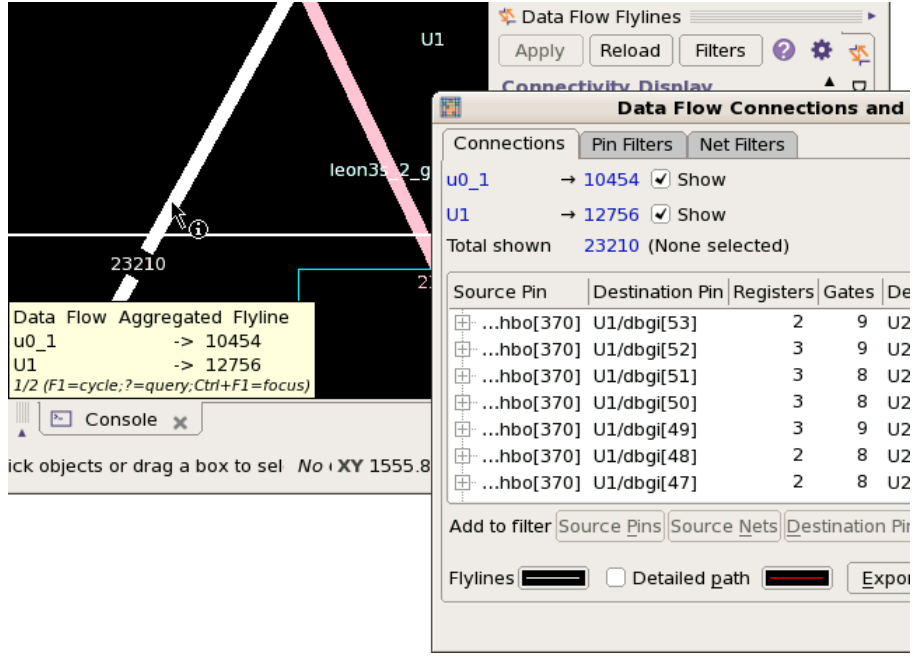
\includegraphics[width=0.92\textwidth]{gui-fig-087.png}
\caption{数据流连接与过滤器}
\label{fig:gui-87}
\end{figure}

Connections 选项卡显示所选飞线内部的连接列表。在该选项卡顶部，工具显示飞线所连接的两个对象的名称，以及从任一对象发出的连接数。若两个对象之间两个方向都有连接，单击对象名右侧的 Show 按钮，把从该对象发出的连接加入列表，或从列表中去掉。

用 Connections 选项卡追踪飞线：
\begin{enumerate}
  \item 单击列表中的一条路径；工具显示该路径的飞线。
  \item 选中 \opt{Detailed path}，显示路径中的全部中间连接；工具为每一段管脚到管脚的连接显示一条红色飞线。
  \item 单击 Source Pins、Source Nets、Destination Pins 或 Destination Nets 按钮，把所选路径复制到相应过滤器；要应用这些过滤器，必须单击 Reload 重新计算飞线。
  \item 单击 ([+]) 按钮展开路径，显示中间连接的源管脚与目标管脚。
  \item 单击列表中代表路径某一段的一项；工具用红色显示该段的详细路径飞线。
  \item 按上箭头键或下箭头键滚动路径，并在版图中高亮不同的段。
  \item 按住鼠标按钮并沿列表向下拖动指针，把路径中的其他段加入选择。
\end{enumerate}

\begin{figure}[htbp]
\centering
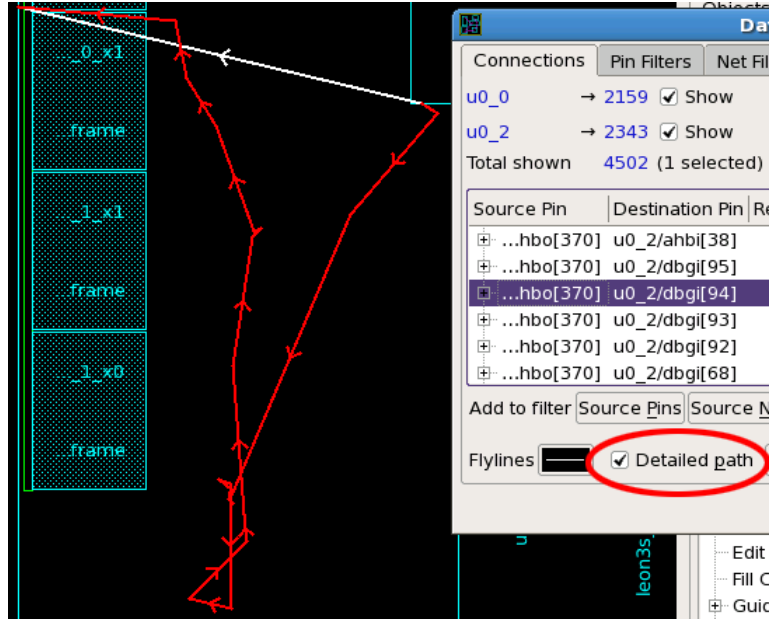
\includegraphics[width=0.92\textwidth]{gui-fig-088.png}
\caption{飞线与详细路径}
\label{fig:gui-88}
\end{figure}

为提高性能，工具可能不会载入全部路径细节。此时，工具在 Detailed Path 列中显示消息 \cmd{Path is not loaded. Double-click to load.}。可以双击该路径以载入它，或单击 Load All Paths 按钮，载入其余全部尚未载入的路径。

要保存列表中各路径的源管脚、目标管脚、寄存器数和门数，并以逗号分隔，单击 Export 按钮。

\subsection{数据流飞线的管脚与线网过滤器}
\label{sec:gui-fly-pinnet}
\subsubsection*{Data Flow Flylines Pin and Net Filters}

要打开 Data Flow Connections and Filters 对话框，单击 Data Flow Flylines 面板中的 Filters 按钮。Pin Filters 与 Net Filters 选项卡包含飞线追踪期间要忽略的管脚列表和线网列表。要向列表添加一项，在 Patterns 框中输入名称并单击 Add。也可以输入与 \cmd{get\_pins} 或 \cmd{get\_nets} 命令兼容的表达式，以指定一个或多个管脚或线网。

在 Pin Filters 或 Net Filters 选项卡中，用右侧按钮修改列表：
\begin{itemize}
  \item 用 Add Selected Pins 按钮或 Add Selected Nets 按钮，把版图中选中的管脚或线网加入列表。
  \item 用 Add Pins of Selected 按钮或 Add Nets of Selected 按钮，加入所选对象的全部管脚或线网。
  \item 用 Remove 按钮从列表中去掉选中项。
  \item 用 Remove All 按钮清空列表。
  \item 用 Write to File 按钮把管脚或线网列表写入文件，每行一项。
  \item 用 Read from File 按钮从文件载入管脚或线网列表。
\end{itemize}

\subsection{用 Tcl 命令分析数据流飞线}
\subsubsection*{Using Tcl Commands to Analyze Data Flow Flylines}

在 Data Flow Flylines 面板中单击 Reload 按钮时，工具打开 Compute Data Flow Flylines 对话框，并提示输入要追踪的级数和最大扇出。也可以直接使用 \cmd{compute\_dff\_connections} Tcl 命令，并向该命令指定选项，以生成寄存器追踪信息。例如，下面的 \cmd{compute\_dff\_connections} 命令生成路径信息，并指定追踪两级寄存器、15 级门，以及最大扇出数为 50。

\begin{lstlisting}
icc2_shell> compute_dff_connections -max_reg 2 -max_gate 15 \
   -max_fanout 50
\end{lstlisting}

用 \cmd{compute\_dff\_connections} 命令追踪飞线之后，使用 \cmd{get\_dff\_connections} 命令返回全部路径，或只返回满足指定条件的路径。默认情况下，该命令返回由 \cmd{compute\_dff\_connections} 命令生成的全部路径的集合。

\begin{noteBox}
用 \opt{-max\_reg} 与 \opt{-max\_gate} 指定的值必须小于或等于 \cmd{compute\_dff\_connections} 命令中对应选项所指定的值。
\end{noteBox}

下面的示例返回由 \cmd{compute\_dff\_connections} 命令提取的特定路径，并返回单条路径的属性。

\begin{itemize}
  \item 返回全部路径。
\begin{lstlisting}
icc2_shell> get_dff_connections
\end{lstlisting}
  \item 返回不含寄存器且不含门的路径。
\begin{lstlisting}
icc2_shell> get_dff_connections -max_reg 0 -max_gate 0
\end{lstlisting}
  \item 返回到达 \cmd{pad[0]} 端口、从 \cmd{pad[0]} 端口出发，以及经过 \cmd{pad[0]} 端口的全部路径。
\begin{lstlisting}
icc2_shell> get_dff_connections -to pad[0]
icc2_shell> get_dff_connections -from pad[0]
icc2_shell> get_dff_connections -through pad[0]
\end{lstlisting}
  \item 返回经过 \cmd{pad[0]} 与 \cmd{u1/u2/o1} 端口的全部路径。
\begin{lstlisting}
icc2_shell> get_dff_connections -through pad[0] -through u1/u2/o1
\end{lstlisting}
  \item 查看集合中单条路径所返回的 \cmd{start.full\_name}、\cmd{end.full\_name} 以及其他属性。
\begin{lstlisting}
icc2_shell> set paths [get_dff_connections -from {pad[6]}]
{{pad[6]::I_ORCA_TOP/I_CONTEXT_MEM ...
icc2_shell> set path [index_collection $paths 0]
{{pad[6]::I_ORCA_TOP/I_CONTEXT_MEM/I_CONTEXT_RAM_0_1/A1[0]}}
icc2_shell> get_attribute $path start.full_name
pad[6]
icc2_shell> get_attribute $path end.full_name
I_ORCA_TOP/I_CONTEXT_MEM/I_CONTEXT_RAM_0_1/A1[0]
icc2_shell> get_attribute $path name
pad[6]::I_ORCA_TOP/I_CONTEXT_MEM/I_CONTEXT_RAM_0_1/A1[0]
icc2_shell> get_attribute $path registers
0
icc2_shell> get_attribute $path gates
10
\end{lstlisting}
\end{itemize}

\subsection{保存与恢复数据流飞线连接数据}
\subsubsection*{Saving and Restoring Data Flow Flylines Connection Data}

退出会话时，工具不保存数据流飞线的连接信息。若希望在以后的会话中使用同一份数据，可以把该信息保存到文件。也可以从已保存的文件中载入，以恢复先前保存的数据流飞线连接信息。

要保存活动视图（active view）当前的数据流飞线连接信息：
\begin{enumerate}
  \item 确认已经计算飞线并载入工具。进一步说明见第~\ref{sec:gui-fly-compute}~节。
  \item 计算飞线之后，用 \cmd{write\_dff\_connections} 命令把数据流飞线连接信息写到文件。
\end{enumerate}

在下面的示例中，工具把数据写到名为 \cmd{dfffile} 的文件。\opt{-force} 选项会覆盖任何同名的已有文件。

\begin{lstlisting}
icc2_shell> write_dff_connections -force -filename dfffile
\end{lstlisting}

要恢复先前保存的数据流飞线连接信息，使用 \cmd{read\_dff\_connections} 命令。

在下面的示例中，工具从名为 \cmd{dfffile} 的文件读取数据流飞线连接信息。

\begin{lstlisting}
icc2_shell> read_dff_connections -filename dfffile
\end{lstlisting}

\begin{itemize}
  \item 将 \opt{-threshold} 选项与 \cmd{read\_dff\_connections} 命令一起使用，以避免当前网表与所要读取的数据流飞线连接不一致时可能出现的问题。该选项的进一步说明见命令手册页。
  \item 若指定文件不在当前工作目录中，工具显示错误消息。
\end{itemize}

若不存在相应附件，将发出 FILE-013 错误。

\begin{lstlisting}
Error: Cannot open file 'filename' for read. (FILE-013)
\end{lstlisting}

要从系统中去掉数据流飞线连接信息文件，使用 \cmd{remove\_dff\_connection\_files} 命令。

在下面的示例中，工具去掉名为 \cmd{dfffile} 的数据流飞线连接文件。要跳过任何消息并以安静模式运行，对该命令使用 \opt{-quiet} 选项。

\begin{lstlisting}
icc2_shell> remove_dff_connection_files -filename dfffile
\end{lstlisting}

\section{寄存器追踪飞线}
\subsection*{Register Tracing Flylines}

IC Compiler II 工具提供 Register Tracing Flylines 工具，用于显示设计中层次、宏单元与端口之间的寄存器连接。可用该工具查看对象之间寄存器连接的飞线，按寄存器级数或扇出限制追踪，显示相连的管脚与端口，并列出路径中的寄存器。要打开 Register Tracing Flylines 面板，选择 \textbf{View > Flylines > Register Tracing}，或单击 Register Tracing Flylines 按钮。Register Tracing Flylines 面板见图~\ref{fig:gui-89}。

\begin{figure}[htbp]
\centering
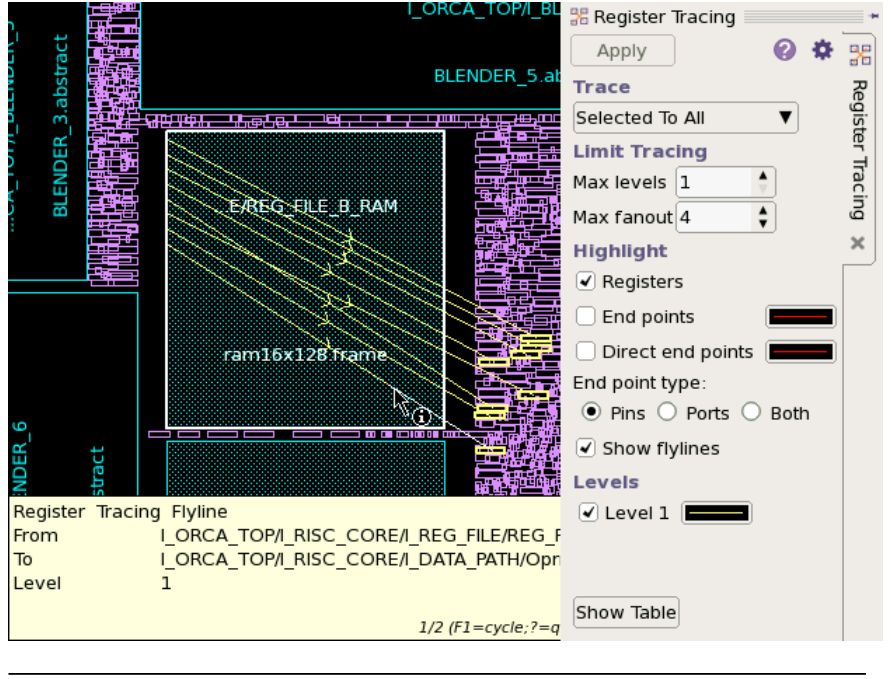
\includegraphics[width=0.92\textwidth]{gui-fig-089.png}
\caption{寄存器追踪飞线面板}
\label{fig:gui-89}
\end{figure}

\subsection{显示飞线}
\subsubsection*{Displaying Flylines}

Register Tracing Flylines 工具在驱动寄存器管脚与接收寄存器管脚之间，为满足指定条件的线网显示飞线。可以按下述方式更改面板中的设置，并单击 Apply 按钮提交更改，从而改变所显示的飞线。
\begin{itemize}
  \item \opt{Trace Selected to All}：按指定级数追踪输出端口，并显示飞线。
  \item \opt{Trace Selected to Selected}：追踪选中对象之间的连接，并显示终点位于其中一个选中对象中的连接。
  \item \opt{Trace All to Selected}：把所有可能的端口和宏单元管脚追踪到所选对象，并且只显示终点位于所选对象中的连接。
  \item \opt{Limit Tracing Max levels}：设置要追踪的最大寄存器级数。
  \item \opt{Limit Tracing Max fanout}：指定停止追踪的扇出级别。
  \item \opt{Highlight registers}：显示并高亮属于寄存器的单元。
  \item \opt{Highlight End points}：以指定的高亮颜色显示并高亮寄存器和端口。
  \item \opt{Highlight Direct End points}：显示并高亮由源管脚（source pin）直接驱动的终点。
  \item \opt{End point type Pins}：只把管脚当作终点。
  \item \opt{End point type Ports}：只把端口当作终点。
  \item \opt{End point type Both}：把管脚和端口都当作终点。
  \item \opt{Show flylines}：切换飞线的可见性。
  \item \opt{All Levels}：切换直到 Limit Tracing 区中所设最大级数的全部追踪级别的可见性。
  \item \opt{Level 1} 等：切换指定级别的可见性。
  \item \opt{Show Table}：显示一个对话框，其中列出满足追踪条件的起点（startpoint）、终点和中间寄存器。单击列表中的一行，在版图中显示对应飞线。单击 Export，把该列表写出。
\end{itemize}

\section{时钟主干规划飞线}
\subsection*{Clock Trunk Planning Flylines}

IC Compiler II 工具提供 Clock Trunk Planning Flylines 工具，用于查看并修改设计中时钟信号的时钟主干（clock trunk）。可用该工具查看各条时钟主干、添加缓冲器、删除缓冲器、检查并修复时钟主干违例，以及为所显示的时钟主干下推（push down）单元。时序信息，例如最差负裕量（worst negative slack，WNS）、TNS 以及其他参数，可以通过为设计中不同的时钟主干规划飞线显示信息提示来查看。要打开 Clock Trunk Planning Flylines 面板，从菜单选择 \textbf{View > Flylines > Clock Trunk Planning}，或单击 Clock Trunk Planning 按钮。Clock Trunk Planning Flylines 面板见图~\ref{fig:gui-90}。

\begin{figure}[htbp]
\centering
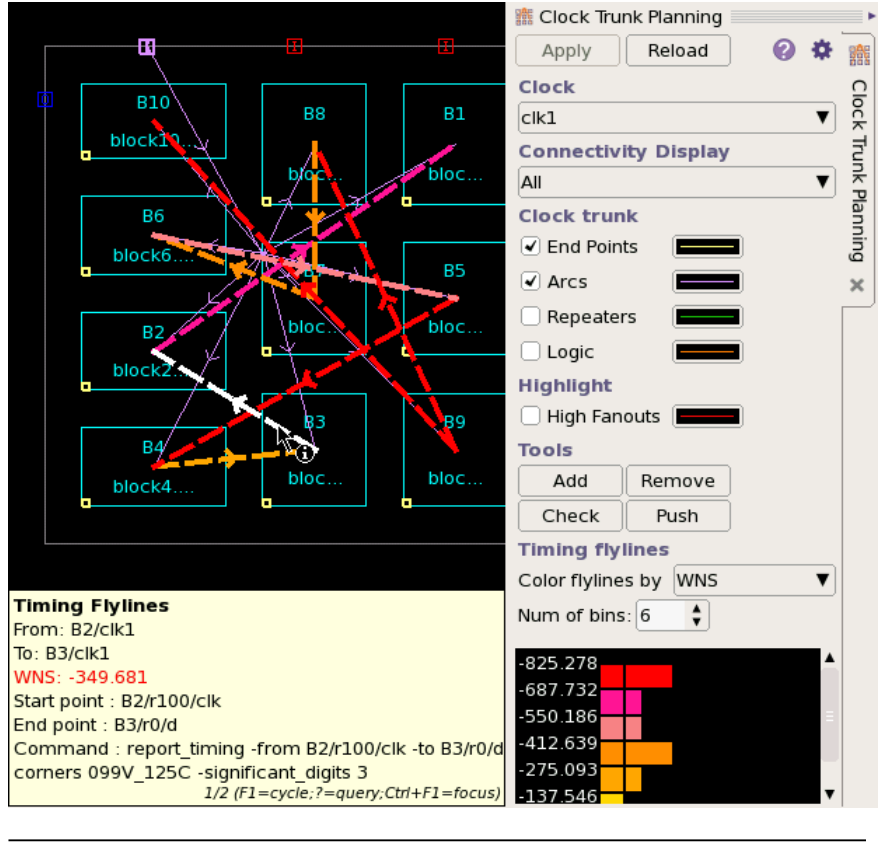
\includegraphics[width=0.92\textwidth]{gui-fig-090.png}
\caption{时钟主干规划控制板}
\label{fig:gui-90}
\end{figure}

\subsection{加载时钟数据}
\subsubsection*{Loading Clock Data}

要把时钟信息载入 Clock Trunk Planning 工具：
\begin{enumerate}
  \item 单击 Reload 按钮。
  \item 在图~\ref{fig:gui-91} 所示的 Reload clock trunk planning 对话框中，选择要加载的时钟。
  \begin{itemize}
    \item 选择 Automatic，加载全部时钟主干。
    \item 选择 Specified，从列表中选择一条或多条时钟主干。按住 Ctrl 键并单击，把时钟加入列表；或按住 Shift 键并单击，一次加入多条时钟。
  \end{itemize}
  \item 单击 OK。
\end{enumerate}

\begin{figure}[htbp]
\centering
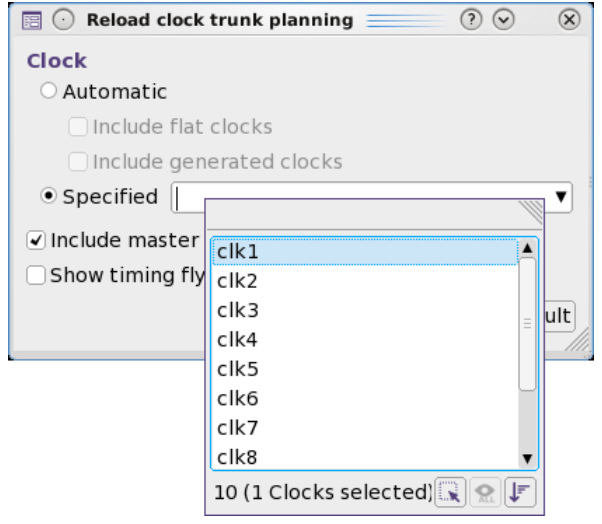
\includegraphics[width=0.92\textwidth]{gui-fig-091.png}
\caption{重新加载对话框}
\label{fig:gui-91}
\end{figure}

工具载入指定的时钟主干。若选择了 Automatic，或选中了多个时钟信号，工具会选中其中一个信号并显示它。要更改所显示的时钟主干，从 Clock 下拉列表中另选一个时钟信号。

\subsection{更改时钟主干高亮}
\subsubsection*{Changing Clock Trunk Highlighting}

用 Clock trunk 区中的控件更改版图里时钟主干元素的颜色。选中元素名旁边的框，即可在版图中显示该元素。单击元素名旁边的色条，并从列表中选择一种颜色，即可更改该时钟主干元素的颜色。
\begin{itemize}
  \item \opt{End Points}：定义时钟终点的颜色。
  \item \opt{Arcs}：定义时钟原点（clock origin）与时钟缓冲器或块之间飞线的颜色。
  \item \opt{Repeaters}：定义中继器（repeater）单元的颜色。
  \item \opt{Logic}：定义逻辑单元的颜色。
  \item \opt{High Fanouts}：定义高扇出线网的颜色。
\end{itemize}

\subsection{添加与删除时钟主干单元}
\subsubsection*{Adding and Removing Clock Trunk Cells}

要在时钟主干上插入时钟缓冲器单元：
\begin{enumerate}
  \item 在控制板的 Clock 框中，选择要插入缓冲器的那条时钟信号的时钟主干。
  \item 在版图中选择要插入缓冲的端口、单元或管脚。该对象必须位于当前选中的时钟主干上。
  \item 单击 Add 按钮。
  \item 在图~\ref{fig:gui-92} 所示的对话框中，选择要插入缓冲的管脚：源管脚、漏管脚（sink pin），或两者都选。
  \item 选中 \opt{Allow on top of blocks} 按钮，允许工具在缓冲器与块重叠时仍然插入缓冲器。
  \item 单击 Add buffer。
\end{enumerate}

工具对第 4 步中所选的每个管脚应用 \cmd{create\_clock\_buffer} 命令，插入一个时钟缓冲器单元。

\begin{figure}[htbp]
\centering
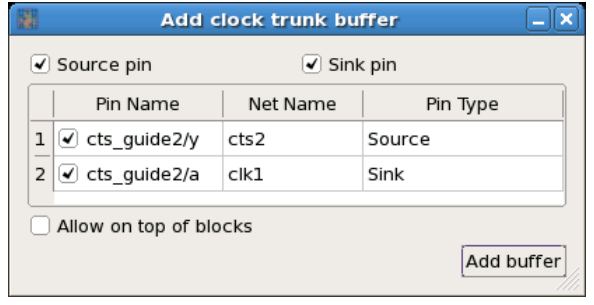
\includegraphics[width=0.92\textwidth]{gui-fig-092.png}
\caption{添加时钟主干缓冲器}
\label{fig:gui-92}
\end{figure}

要去掉一个或多个时钟缓冲器单元：
\begin{enumerate}
  \item 在版图中选中这些单元。
  \item 单击 Remove 按钮。
\end{enumerate}

\subsection{显示块之间的时序飞线}
\subsubsection*{Displaying Timing Flylines Between Blocks}

Clock Trunk Planning 工具可以显示设计中块之间的时序飞线。在控制板底部附近 Timing flylines 区的 Color flylines by 框中，选择一种时序度量：WNS、WNS(OCV)、TNS、Slack、Slack(OCV)、Paths 或 VioPaths\&TNS。其中 OCV 为片上变异（on-chip variation），Slack 为裕量（slack）。工具对路径分档，按档把飞线加到版图上，并在控制板底部显示数值直方图（histogram）。要更改所显示的档数，在 Num of bins 框中设置新值。

要从版图中去掉时序飞线，在 Color flylines by 框中选择 None。
